\subsection{Q-Learning}
%
Q-Learning ist ein modellfreier Algorithmus für das Erlernen der optimalen Entscheidungsfindung in der RL-Umgebungen. Der Algorithmus wurde 1989 von Chris Watkins in seiner Doktorarbeit eingeführt und hat sich als einer der beliebtesten Algorithmen im Bereich des RL-Umgebungen etabliert \cite{morales2020grokking}. Anstelle eines Übergangsmodells wird eine .direkt aktualisiert, die die Qualität jeder möglichen Aktion in einem bestimmten Zustand repräsentiert \cite{russell2021ai}.
%
\paragraph{Mathematische Grundlagen}
%
Die Aktualisierung der Q-Werte \( Q(s, a) \) erfolgt anhand der Bellman-Gleichung:
\[
		Q(s, a) \leftarrow Q(s, a) + \alpha \left[ R(s, a, s') + \gamma \max_{a'} Q(s', a') - Q(s, a) \right]
		\label{eq: update q learning}
\]
wobei \( s \) der aktuelle Zustand, \( a \) die gewählte Aktion, \( s' \) der neue Zustand, \( R(s, a, s') \) die unmittelbare Belohnung, \( \alpha \) die Lernrate und \( \gamma \) der Abschlagfaktor ist \cite{russell2021ai}.
%
\paragraph{Pseudocode}
Der Pseudocode für den Q-Learning-Algorithmus könnte wie folgt aussehen:\\
%
\begin{algorithmic}
		\STATE Initialize $Q(s, a)$ for all states and actions
		\STATE Set parameters $\alpha$ and $\gamma$
		%
		\FOR{each episode}
		\STATE Initialize state $s$
		\WHILE{$s$ is not a terminal state}
		\STATE Choose action $a$ based on policy (e.g., epsilon-greedy) derived from $Q(s, a)$
		\STATE Take action $a$, observe reward $r$ and new state $s'$
		\STATE Update Q-value:
		\STATE $Q(s, a) \gets Q(s, a) + \alpha \cdot (r + \gamma \cdot \max(Q(s', a')) - Q(s, a))$
		\STATE $s \gets s'$  \# Move to the new state
		\ENDWHILE
		\ENDFOR
\end{algorithmic}
%
Dieser Algorithmus benötigt keine Modellierung der Umgebung und ist daher besonders nützlich in komplexen oder unbekannten Umgebungen \cite{morales2020grokking}. Es handelt sich um ein "Off-Policy"-Verfahren, was bedeutet, dass es die optimale Q-Funktion lernt, unabhängig von der während des Lernens verwendeten Richtlinie \cite{morales2020grokking}.

Die sogenannte Heatmap in Abbildung \ref{fig:grid_world_q_learning} visualisiert die Q-Werte, die der Agent in jedem Zustand der Rasterwelt zugewiesen hat. Die Farbgebung illustriert, wie Q-Learning durch Interaktion mit der Umgebung diese Werte optimiert, indem es Belohnungen maximiert, was durch die Bellman-Gleichung mathematisch fundiert ist. Dieser Prozess des stetigen Aktualisierens der Q-Werte, die die erwarteten zukünftigen Belohnungen für jede Aktion in jedem Zustand repräsentieren, zeigt die modellfreie Natur des Q-Learning-Algorithmus und seine Fähigkeit, optimale Strategien zu erlernen, auch wenn die genaue Dynamik der Umgebung unbekannt ist. Die in Abbildung \ref{fig:grid_world_q_learning} dargestellten Informationen ergänzen somit die theoretischen Konzepte, die in diesem Abschnitt diskutiert wurden, indem sie ein konkretes Beispiel für die Anwendung von Q-Learning in einer simulierten Umgebung bieten \cite{klein_abbeel_cs188}.
%
%
\begin{figure}[htbp]
		\centering
		% erstes Bild
		\begin{minipage}[b]{0.48\linewidth}
				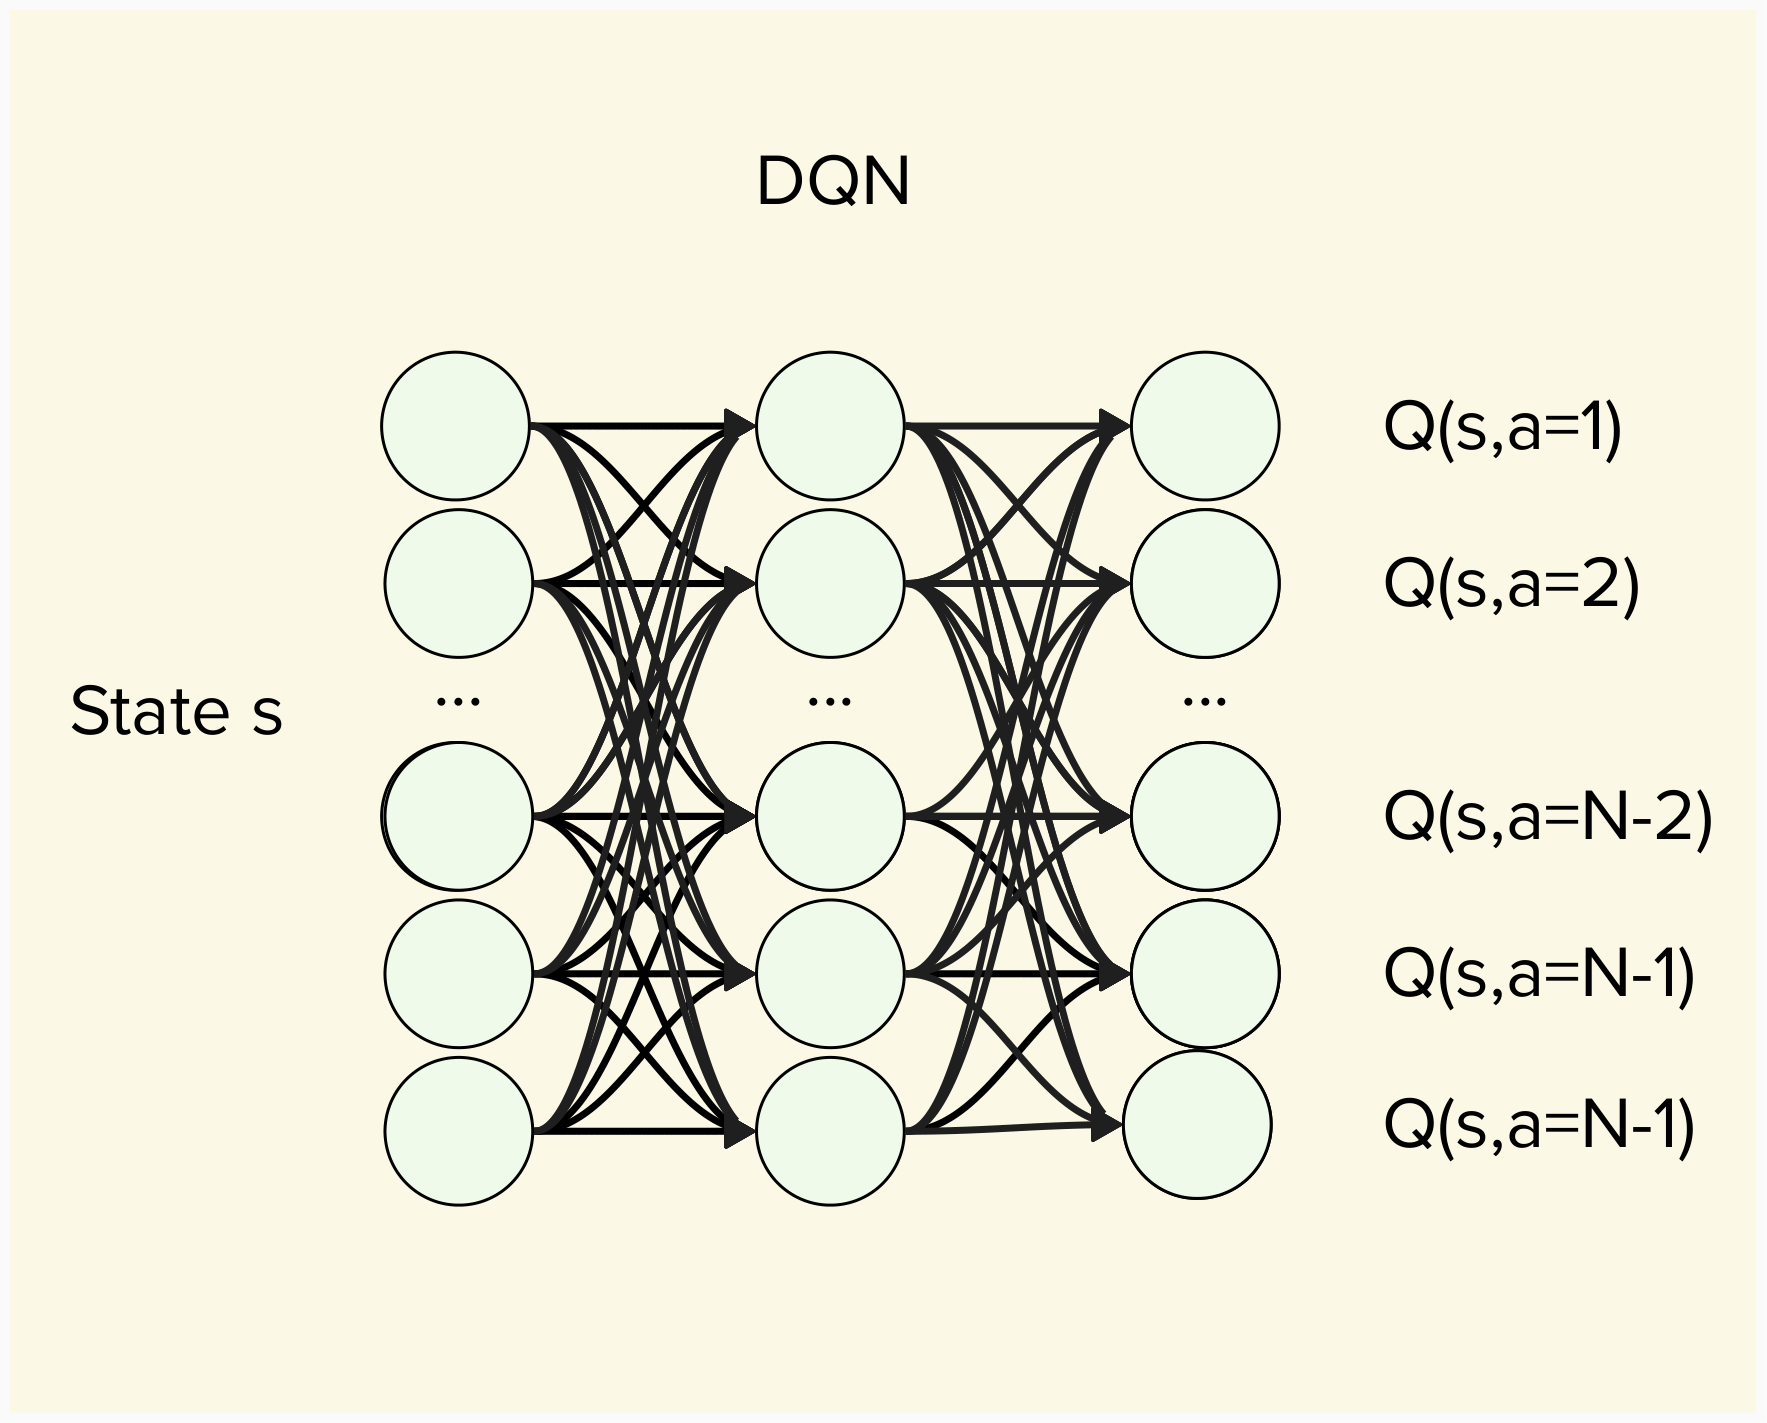
\includegraphics[width=\linewidth]{2Grundlagen/33grid_world_q_learning.png}
				\caption{Schematische Darstellung eines Deep Q-Networks (DQN), das für RL-Umgebungen verwendet wird.}
				\label{fig:dqn}
		\end{minipage}
		\hfill % Dies sorgt für Abstand zwischen den Bildern
		% zweites Bild, angehoben um 50pt
		\raisebox{1pt}[0pt][0pt]{%
				\begin{minipage}[b]{0.48\linewidth}
						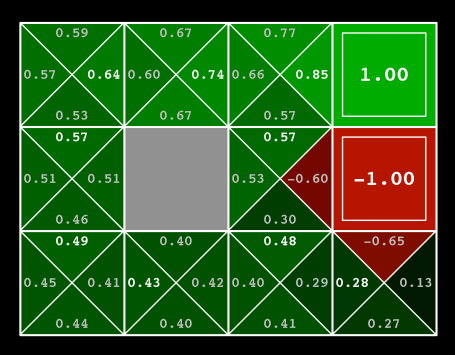
\includegraphics[width=\linewidth]{2Grundlagen/33Q_Values.png}
						\caption{Darstellung einer Heatmap von Q-Werten in einer Rasterwelt.}
						\label{fig:grid_world_q_learning}
						\cite{klein_abbeel_cs188}
				\end{minipage}%
				}
\end{figure}

\paragraph{Das $\epsilon$-greedy Verfahren im RL-Umgebungen}
\begin{equation}
		a = 
		\begin{cases}
				\underset{a}{\mathrm{argmax}}\ Q(s,a) & \text{mit Wahrscheinlichkeit } 1 - \epsilon, \\
				\text{eine zufällige Aktion} & \text{mit Wahrscheinlichkeit } \epsilon.
		\end{cases}
		\label{eq:epsilon_greedy}
\end{equation}


\paragraph{Deep Q-Learning}

Der Kernunterschied zwischen Q-Learning und Deep Q-Learning (DQL) liegt in der Methodik der Approximation der Q-Werte, die im Zentrum beider Ansätze steht. Klassisches Q-Learning nutzt eine Q-Tabelle, um Werte für Zustands-Aktions-Paare zu speichern, was bei einer begrenzten Anzahl von Zuständen und Aktionen gut funktioniert. Jedoch wird diese Methode unpraktikabel in komplexen, hochdimensionalen Umgebungen. Hier kommt DQL ins Spiel, das neuronale Netze verwendet, um diese Werte effizient zu schätzen \cite{morales2020grokking}. 

Wie Abbildung \ref{fig:dqn} veranschaulicht, ermöglicht die Verwendung von tiefen neuronalen Netzen in einem Deep Q-Network (DQN), eine effektive Handhabung von Situationen mit einer hohen Anzahl von Zuständen, die über das Fassungsvermögen einer herkömmlichen Q-Tabelle hinausgehen. Diese fortgeschrittenen Netzwerke sind in der Lage, direkt aus rohen visuellen Eingaben zu lernen und entwickeln im Laufe der Zeit eine verfeinerte Q-Funktion, welche die Entscheidungsfindung des Agenten verbessert. Diese Verbesserung wird durch den Einsatz von Deep Learning-Techniken erreicht, die es dem DQN ermöglichen, abstrakte Repräsentationen für die Entscheidungsfindung zu lernen und zu nutzen, was eine signifikante Verbesserung gegenüber traditionellen Q-Learning-Techniken darstellt \cite{brunton2019data}.


\paragraph{Exploration versus Exploitation}
\label{sec: Exploration versus Exploitation}

Die Balance zwischen Exploration und Exploitation ist essentiell für die Effektivität von lernenden Agenten im Q-Learning, die sich im Laufe ihrer Interaktion mit der Umgebung stetig anpassen müssen.

Durch die Anwendung des \(\epsilon\)-greedy Verfahrens \ref{eq:epsilon_greedy} im RL-Umgebungen wird ein Kompromiss zwischen der Erforschung unbekannter Aktionen und der Ausnutzung bekannter Strategien gefunden. Dies ermöglicht es einem Agenten, sowohl Neues zu entdecken als auch bewährte Taktiken einzusetzen, um den unmittelbaren Gewinn zu maximieren \cite{SuttonBarto2018}.

Die Dynamik von \(\epsilon\) spielt eine wichtige Rolle: Zu Beginn des Lernprozesses fördert ein höheres \(\epsilon\) die Exploration. Mit zunehmender Erfahrung sollte \(\epsilon\) jedoch sinken, was den Übergang zur gezielten Exploitation bewirkt \cite{morales2020grokking}.

Simulated Annealing erlaubt es, unter bestimmten Bedingungen auch Verschlechterungen des aktuellen Zustands zu akzeptieren. Dies wird durch die "Temperatur", einen Metaparameter, ermöglicht, der analog zur physikalischen Temperatur in der Metallurgie die Wahrscheinlichkeit für das Akzeptieren schlechterer Zustände bestimmt \cite{russell2021ai}. Im Metallurgieprozess bezeichnet Annealing den Vorgang, bei dem Metalle und Glas erhitzt und dann langsam abgekühlt werden, um eine stabile, kristalline Struktur zu erlangen \cite{russell2021ai}.
\label{sec:Simulated Annealing}

Simulated Annealing beginnt mit einer hohen "Temperatur", die es dem Algorithmus ermöglicht, lokale Minima zu verlassen, indem temporär schlechtere Lösungen akzeptiert werden. Mit der Zeit wird die Temperatur reduziert, wodurch der Algorithmus sich einem globalen Optimum annähert. Eine ähnliche Vorgehensweise findet sich im \(\epsilon\)-greedy Verfahren, bei dem \(\epsilon\), ein Parameter, der die Exploration im Verhältnis zur Exploitation steuert, allmählich verringert wird. Wie bei der kontrollierten Abkühlung, die Materialien in eine stabilere Struktur überführt, reduziert das Senken von \(\epsilon\) im Laufe der Zeit die Neigung zur Erkundung und fördert eine zunehmend spezialisierte Nutzung der besten bekannten Handlungsoptionen \cite{russell2021ai}.

Durch die methodische Reduktion von \(\epsilon\) wird vermieden, dass der Lernprozess in suboptimalen Lösungen verharrt. Stattdessen bleibt die Möglichkeit erhalten, bessere Aktionen zu entdecken und zu nutzen, was zu einer effektiveren und effizienteren Suche führt \cite{russell2021ai}.

Die Feinabstimmung von \(\epsilon\) ist entscheidend, da eine nicht angepasste Rate entweder zu wenig Exploration oder zu verzögerter Optimierung führen kann \cite{morales2020grokking}.



\paragraph{Replay Buffers}
\label{sec:Replay Buffers}

Replay Buffers verringern die Korrelation aufeinanderfolgender Erfahrungen und fördern so die Stabilität beim Lernen von RL-Agenten \cite{morales2020grokking}. Sie speichern eine Sammlung von Erfahrungstupeln aus unterschiedlichen Policies und Trajektorien und ermöglichen eine effektivere Trainingsmethode durch zufällige Stichprobenziehung, was die Netzwerkaktualisierungen diversifiziert \cite{morales2020grokking}.

Mathematisch wird der Replay Buffer wie folgt definiert \cite{morales2020grokking}:
\begin{equation}
		\mathcal{D} = \{ e_t = (s_t, a_t, r_t, s_{t+1}, d_t) \mid t \in \{1, \ldots, T\} \}
\end{equation}

Sampling aus dem Replay Buffer erfolgt per Zufallsauswahl ohne Zurücklegen, um einen Minibatch von \( n \) Erfahrungen zu generieren:
\begin{equation}
		\mathcal{B} = \{ e_i \mid e_i \in \mathcal{D}, i \in \mathcal{I} \}
		\label{eq:replay buffer}
\end{equation}
wobei \( \mathcal{I} \subset \{1, \ldots, T\}, \quad |\mathcal{I}| = n \).

Die Kapazität des Buffers und das gleichförmige Sampling sorgen für ein diversifiziertes Lernen und vermeiden lokale Optima \cite{morales2020grokking}. Die effektive Nutzung eines Replay Buffers erfordert eine ausreichende Kapazität, die typischerweise zwischen 10.000 und 1.000.000 Erfahrungen variiert \cite{morales2020grokking}. Ein priorisiertes Sampling könnte eine intelligentere Auswahlmethode darstellen, die eine ausgewogenere Lernumgebung fördert \cite{morales2020grokking}.
%
\paragraph{Fortgeschrittene Anpassungsfähigkeit und Lernmechanismen in Tiefen Q-Netzwerken (DQN) und ihre Bedeutung in der Entwicklung Künstlicher Intelligenz}
%
Die Tiefen Q-Netzwerke (DQN) haben sich als revolutionär in der Landschaft des maschinellen Lernens erwiesen. Mit ihrer Fähigkeit, eine Policy direkt aus rohen Pixeln zu lernen, signalisierte das DQN einen Wendepunkt in der Forschung von Reinforcement Learning (RL). Wie in \cite{morales2020grokking} dargestellt, hat das DQN die Tür zu einer Vielzahl von Forschungsinnovationen geöffnet und zu Beginn eine Leistung demonstriert, die auf menschenähnlichem Niveau auf einem Atari-Benchmark lag. Es ist erwähnenswert, dass trotz der Weiterentwicklungen DQN in seiner ursprünglichen Form nicht mehr als Primärwahl für aktuelle Anwendungen gilt, es bleibt jedoch ein Schlüsselelement unter den bestperformenden DRL-Agenten.
%
Die Fähigkeit des DQN, optimale Policy aus einer komplexen Umgebung wie der eines Atari-Spiels zu extrahieren, ist vergleichbar mit der Navigation in einem sich ständig verändernden Labyrinth, auf der Suche nach dem optimalen Weg (\cite{russell2021ai}). Die Anwendung der neuronalen Netze, speziell die tiefen Architekturen, ermöglicht es dem DQN, abstrakte Repräsentationen zu erlernen und diese für die Entscheidungsfindung zu nutzen.
%
Eine Herausforderung, auf die in \cite{SuttonBarto2018} hingewiesen wird, ist jedoch, dass DQN bei Spielen wie Montezuma's Revenge, die tiefergehende Planung erfordern, an seine Grenzen stößt. Obwohl DQN wesentliche Fortschritte im maschinellen Lernen gezeigt hat, verbleiben Herausforderungen in seiner Fähigkeit, komplexe Planungsaufgaben zu meistern.
%
Das beeindruckende Potenzial der DQN-Methode wurde weiterhin durch das System AlphaGo von DeepMind illustriert, das tiefes RL verwendete, um menschliche Experten im Go-Spiel zu schlagen, einem Spiel, das für seine immense Anzahl möglicher Positionen bekannt ist und weit über das hinausgeht, was traditionelle Spiele bieten (\cite{russell2021ai}). Dies bestätigt, dass trotz der Herausforderungen, DQN und seine Weiterentwicklungen ein hohes Maß an Anpassungsfähigkeit und Lernfähigkeit aufweisen, das es ihnen ermöglicht, auch in komplexen Umgebungen zu bestehen.
%
Im Licht dieser Quellen lässt sich zusammenfassen, dass DQN und dessen Erweiterungen ein bedeutsames Fundament für die Entwicklung von lernenden Agenten bieten, das sowohl die Forschung als auch praktische Anwendungen weiterhin beeinflusst.
%

\paragraph{Grenzen von Deep Q-Learning in kontinuierlichen Aktionsräumen}
Deep Q-Learning zeigt zwar in diskreten Aktionsräumen eine beeindruckende Leistung, stößt aber bei der Diskretisierung von kontinuierlichen Aktionsräumen auf bedeutende Herausforderungen. Die Notwendigkeit, kontinuierliche Aktionen in diskrete Schritte zu unterteilen, kann zu einem Verlust an Präzision und einer Verschlechterung der Leistung führen, insbesondere in Bereichen wie der Robotik, wo fein abgestimmte Kontrollaktionen erforderlich sind. Diese Limitation kann auch durch die Verwendung von Bewegungsprimitiven anstatt von niederstufigen Aktionen gemildert werden, was zwar das Lernen beschleunigt, aber die Bandbreite der Verhaltensweisen, die der Roboter lernen kann, einschränkt \cite{russell2021ai}. Weiterhin kann die Diskretisierung zu instabilen Steuerungsvorgängen führen, was insbesondere in sicherheitskritischen Systemen wie autonomen Fahrzeugen problematisch ist \cite{Wu2018AggregatedMultiDDPG}. Zusätzlich wird die Anwendung von Deep Q-Learning durch die erhöhte Berechnungskomplexität und Schwierigkeiten bei der Konvergenz in großen Zustandsräumen eingeschränkt \cite{russell2021ai}.



